\documentclass{comjnl}

\usepackage{amsmath}
\usepackage{hyperref}
%\usepackage[margin=0.5in]{geometry}
\usepackage{float}
\newcommand*\chem[1]{\ensuremath{\mathrm{#1}}}

%% These two lines are needed to get the correct paper size
%% in TeX Live 2016
\let\pdfpageheight\paperheight
\let\pdfpagewidth\paperwidth

%\copyrightyear{2009} \vol{00} \issue{0} \DOI{000}

\begin{document}

\title[Superconductivity in Rutherford MgB2 Cables and cuprate/manganite multilayer]{How superconductivity in Rutherford MgB2 Cables and cuprate/manganite multilayer is affected by external factors}
\author{Even M. Nordhagen}
\affiliation{Computational physics group, Department of Physics, University of Oslo, Oslo, Norway} \email{evenmn@fys.uio.no}

\shortauthors{E. M. Nordhagen}
 
\received{00 November 2017}
\revised{00 Month 2017}


%\category{C.2}{Computer Communication Networks}{Computer Networks}
%\category{C.4}{Performance of Systems}{Analytical Models}
%\category{G.3}{Stochastic Processes}{Queueing Systems}
%\terms{Internet Technologies, E-Commerce}
\keywords{Superconductivity; Rutherford cable; Cuprate; Manganite; YBCO; Transport measurements; Magneto Optical Imaging}


\begin{abstract}
We investigate the superconductive properties of 12 twisted Rutherford \chem{MgB_2} cables and 10 layers of \chem{Pr_{0.5}La_{0.2}Ca_{0.3}MnO_3/YBa_2Cu_3O_7} (PLCMO/YBCO) using transport measurements and magneto-optical imaging, with the former as the main focus. The transport measurements were done carefully, where we studied how the resistance and current through the sample was affected by the temperature. Liquid helium was used to cool down the sample to lower temperatures (min 3.7K), and for a bit higher temperatures we used liquid nitrogen (min 77K).  Furthermore magneto-optical imaging was inducted only for the Rutherford tape.
\end{abstract}

\maketitle


\section{Introduction}
Humans are burning huge amounts of oil to get energy, essentially for electricity or transport usage. Exactly how much oil is remaining on Earth is unknown, and how much we can make use of depends on the future technology. Anyway what is sure is that it will not last forever, and we need to find new, probably renewable, energy sources. What if we could find a renewable energy carrier which was so cold that it could cause superconductivity at the same time? We do not need to search further, the solution is liquid hydrogen! When hydrogen reacts with oxygen, we get water, which is 100\% renewable, at the same time as liquid hydrogen has a temperature of $20K$.

To improve the hydrogen economy, we need a material which is superconducting above $20K$ and can be made in large scales. For a long time, this material was unable, but in 2001 a group of Japanese scientists found that \chem{MgB_2} has transition temperature of $T_c=39K$, which is the highest of all known metallic superconductors \cite {jsap}\cite {nature}. This again gave hope for possible large-scale applications of superconductors using cryogen-free technology. 

We are going to study a Rutherford tape consisting of cables with cores of \chem{MgB_2}. Rutherford cables are frequently used to generate magnetic fields in particle accelerators, and were first developed at the Rutherford Laboratory, hence the name \cite {fnal}. Our sample was sent from Spain, and we will return the results as soon as they are ready. Maybe we participate in developing the next generation particle accelerators?

Moreover we have examined the superconducting properties of a YBCO multilayer sample. YBCO has status as the first material to be found superconducting above the temperature of liquid nitrogen, which generated major optimism for superconductivity when it was discovered in 1987 \cite{harvard}, with its critical temperature of $T_c=93K$. 

\section{Theory}\label{Sec:Theory}
Superconductive materials have two main properties: They are resistance-free conductors under a critical temperature $T_c$ and magnetic field cannot penetrate the material under the same temperature $T_c$. The methods we gonna make use of both these main properties. Perhaps the easiest way to find the resistance of a sample is to connect the sample to a power supply and measure the voltage difference, $U$, between two points. The resistance can then be calculated by Ohm's law $U=RI$, given the current $I$. This is known as a four-point measurement or four-terminal sensing, and is widely used in transport measurements. No voltage drop corresponds to zero resistance. In figure (\ref{fig:4point}) one can find a sketch of a four-point measurement. It is crucial that all the contacts are made all the way across the sample, such that the current is uniformly distributed. It should neither be able to avoid the potential contacts.
\begin{figure}[h]
\centering
\includegraphics[width=70mm]{4point.png}
\caption{General 4-point method with four contacts. The two outermost (I1 and I2) are connected to current cables, such as current flows through the sample while the innermost contacts (U1 and U2) are connected to potential cables. See text for further reading. \label{fig:4point}}
\end{figure}

In some cases it is appropriate to use more advanced techniques, for instance when the sample structure is not uniform in every direction. Then we might want to measure the resistance in various directions, but without disturbing the samples with more contacts than necessary. By placing the contacts in each corner, we can reuse the contacts when "turning" the sample, known as the monogomery, illustrated in figure (\ref{fig:4corner}). 

\begin{figure}[h]
\centering
\includegraphics[width=60mm]{4corner.png}
\caption{The 4-corner measurement is used in the monogomery technique to study the anisotropy of a sample. Contact U1 and U2 are connected to a voltmeter, while contact I1 and I2 are the current contacts. \label{fig:4corner}}
\end{figure}

\subsection{Magneto-Optical Imaging (MOI)}
Our eyes are not able to see magnetism, but with a MOI apparatus we can take pictures of a superconductor and decide if a sample is superconducting, using the elementary magnetic property discussed in section \ref{Sec:Theory}. The method is quite in-complicated where light is reflected by a Faraday crystal on top of the sample. If the Faraday crystal is affected by a magnetic field, it will polarize the light, and it will later be separated out by a polarization filter, as shown in figure (\ref{fig:MOI}). The idea is that all the light will go through the filter as long as the sample is not superconducting. Alternatively if the sample is superconducting, we will get no light passing in the superconducting area. Not only can MOI detect superconductivity, but we can also see exactly where the material is superconducting, which is convenient for non-homogeneous materials. 
\begin{figure}[h]
\centering
\includegraphics[width=80mm]{moi.png}
\caption{A simple sketch of a MOI apparatus, which consists of two polarizators, a couple of mirrors, a magnet, a Faraday crystal and a photo detector. See text to find out how it works. \label{fig:MOI}}
\end{figure}

\section{Experiments}\label{Sec:Experiments}
Now as the theory behind the methods is introduced, we are ready to see how the experiments actually were done. Our samples are the Rutherford tape consisting of 12 cables and the YBCO multilayer. Only the former was used in Magneto-Optical imaging, while we did transport measurements on both. 

\subsection{Rutherford tape}
A Rutherford cable is a cable consisting of multiple layers of superconducting materials. Our sample has a core of \chem{MgB_2} (with $39K$ as the transition temperature) covered by a layer of Niobium, which is another superconductor with critical temperature $7K$. We then expect really low total resistance below $7K$, a little more resistance between $7K$ and $39K$, and no superconductivity above $39K$. The Niobium layer is again covered the non-superconducting metal Cu10Ni, probably to protect the cables. A corss section optical image is shown in figure (\ref{fig:rutherford2}).
\begin{figure}[h]
\centering
\includegraphics[width=50mm]{rutherford2.jpg}
\caption{Cross section of the Rutherford tape, showing the \chem{MgB_2} core (dark) apparently covered by a gray layer. Both the outermost layers look gray and it is hard to differ them on an optical image. The picture was taken after polishing, as we can see on some of the cables. \label{fig:rutherford2}}
\end{figure}

\subsubsection{Transport Measurements}
The transport measurements on the Rutherford tape were done using 4-point connection defined in the theory. We used liquid helium to cool down the sample, because liquid nitrogen would not be cold enough. First we placed the sample on the sampleholder, and connected current and potential contacts. The contacts were made of Indium (In) since it is a good conductor and easy to distribute, see figure(\ref{fig:sampleholder}) for a picture after the cables are connected. Then we had to attach the sample using adhensive tape. This tape worked as an isolator for the potential and current cables at the same time. To ensure the tape would not loosen, we strapped a thread around it. 

\begin{figure}[h]
\centering
\includegraphics[width=70mm]{sampleholder.jpg}
\caption{The Rutherford tape placed on sample holder where all the four cables are connected.  \label{fig:sampleholder}}
\end{figure}

Further we added heat isolation to make the temperature changes more smooth. First a finger was cut of a blue vinyl glow, and attached around the sample with tape. Unfortunately we found this to be too well isolated, so we tried with a transparent finger. This worked better, but the temperature changes were not always as smooth as desired. A vinyl finger would also protect the sample in case it was dipped in the liquid helium. Moreover we struggled with several other isolation mechanisms, not always successful. 

After the sample holder was prepared, we could go on measure the resistance as the sample was sinked into the liquid helium container. We measured both on the way down and on the way up, and sometimes we went up and down around critical temperature to see if we got hysteresis and eventually how big it was. In section \ref{Sec:Results} the results are presented.

\subsubsection{Magneto-Optical Imaging (MOI)}
Before the MOI analysis was done, we polished the sample to get the Faraday crystal closer to the superconducting part. This was done by a rotating sandpaper, and a image is shown in figure (\ref{fig:rutherford1}). Thereafter we cleaned it and placed it on the sample holder using vacuum fat which becomes sticky in vacuum. The Faraday crystal can not be attached to the sample in any way, so we needed stabilizators to make sure that it did not fall of the sample. When the sample was prepared, we could prepare for the experiment. The step were 1. Place sampleholder with sample inside MOI machine, 2. make vacuum, 3. cool down. 
\begin{figure}[h]
\centering
\includegraphics[width=70mm]{rutherford1.jpg}
\caption{This is how the Rutherford tape looked after polishing, and one looks carefully it is not uniformly polished. Especially the lower part is not ideal. \label{fig:rutherford1}}
\end{figure}
\begin{figure}[h]
\centering
\includegraphics[width=50mm]{sampleholder2.jpg}
\caption{Rutherford cable placed on the MOI sample holder, covered by a Faraday crystal. A watchful eye will see the stabilizators to keep the Faraday crystal on top. \label{fig:sampleholder2}}
\end{figure}

\subsection{PLCMO/YBCO multilayer}
We have a sample consisting of 10 extremely thin layers of YBCO \chem{YBa_2Cu_3O_7} with PLCMO \chem{Pr_{0.5}La_{0.2}Ca_{0.3}MnO_3} in between. YBCO is superconducting of $93K$, and we can therefore study the superconducting properties even in liquid nitrogen. PLCMO is not a superconductor, and with thickness 20nm it is thicker than the YBCO layers which are 7nm each. 

\subsubsection{Transport measurements}
For this sample the transport measurements were conducted using the 4-corner measurements, which makes us able to study the anisotropy. In figure (\ref{fig:multilayer}) one see how the cables were connected to the sample.
\begin{figure}[h]
\centering
\includegraphics[width=60mm]{multilayer.png}
\caption{The cables are connected to the YBCO multilayer using the 4-corner connections. \label{fig:multilayer}}
\end{figure}
We later turned the sample, i.e, all the cables were connected to the neighbor contacts and we repeated the measurements, referred to as the monogomery technique. 

First we investigated how the superconductive properties behaved in low temperature using liquid helium as the cooling medium, but after a few days with measurements we ran out of liquid helium and had to use liquid nitrogen. When using liquid helium, the container was equiped with a holder which made it easy to sink the sample into the helium slowly and lift it carefully. We did not have this equipment for the liquid nitrogen container, and had to develop our own patent. A image of this patent in use is found in figure (\ref{fig:patent}). The sample was dipped into a beaker containing liquid nitrogen as showed in figure (\ref{fig:nitrogen}). 
\begin{figure}[h]
\centering
\includegraphics[width=60mm]{patent.jpg}
\caption{Our own patent to be able to increase and decrease the bar with the sample smoothly. On the flour you can spot the beaker with liquid nitrogen. \label{fig:patent}}
\end{figure}
\begin{figure}[h]
\centering
\includegraphics[width=40mm]{nitrogen.jpg}
\caption{Beaker with nitrogen. \label{fig:nitrogen}}
\end{figure}
Also for this sample we did measurements both on the way down and on the way up, but with this method it was difficult to increase the sample such that the temperature change was constant. Instead of moving it slowly upwards, we laid the sample on a table and did measurements when it approached room temperature. To keep smooth temperature changes, it was pushed into a thick, isolating glow, as shown in figure (\ref{fig:glow}).
\begin{figure}[h]
\centering
\includegraphics[width=40mm]{glow.jpg}
\caption{A thick glow was used to heat the sample slowly. \label{fig:glow}}
\end{figure}


\section{Results}\label{Sec:Results}
As section \ref{Sec:Experiments} indicates, we have studied Rutherford cable by transport measurements with a 4-point connection, and we also magneto-optical imaging has been used to reveal the superconducting properties of the sample. Additionally the YBCO multilayer has been investigated by transport measurements. The experiments are detailed in section \ref{Sec:Experiments}.

\subsection{Rutherford cable}
\subsubsection{Transport measurements}
All the transport measurements done using liquid helium as cooling medium. In figure (\ref{fig:rutherfordRTallI}) and (\ref{fig:rutherfordRTlowI}) you can find resistance plotted as function of temperature for low currents in the temperature range 160K to 25K and around the critical temperature respectively. 
\begin{figure}[h]
\centering
\includegraphics[width=70mm]{Rutherford_RT_all_T_low_I.png}
\caption{Resistance plotted as function of temperature from 160K to 25K. The dark graph is 0.2A, the blue graph is 0.5A and the pink graph is 0.7A. \label{fig:rutherfordRTallI}}
\end{figure}
\begin{figure}[h]
\centering
\includegraphics[width=70mm]{Rutherford_RT_low_I.png}
\caption{Resistance plotted as function of temperature around critical temperature. The dark graph is 0.2A, the blue graph is 0.5A and the pink graph is 0.7A. \label{fig:rutherfordRTlowI}}
\end{figure}
As we can see in figure (\ref{fig:rutherfordRTallI}, all the curves seem to follow almost the same path, but with more spread for higher temperatures. We get transition of 37K, as expected, and on the zoomed-in plot in figure (\ref{fig:rutherfordRTlowI}) one can see that we got trasition for the highest temperature at 0.5A, followed by 0.7A and 0.2A. This is suspicious since higher currents should give us transition at lower temperature. Furthermore we study the hysteresis in figure (\ref{fig:rutherfordRT}) where resistance is plotted against the temperature for 0.05A, 0.1A and 0.3A. We can immediately see that the graphs are ordered correctly in this care, with 0.05A as the graph with transistion at highest temperature.
\begin{figure}[h]
\centering
\includegraphics[width=70mm]{Rutherford_RT.png}
\caption{Resistance as function of temperature around critical temperature. The red graph corresponds to 0.05A, the black corresponds to 0.1A and the blue one corresponds to 0.3A. See text for futher description. \label{fig:rutherfordRT}}
\end{figure}


\subsubsection{Magneto-optical imaging}
We did magneto-optical imaging as described in section \ref{Sec:Experiments}, and we got the image presented in figure (\ref{fig:moi2d1}) when a current of 3.4A was sent through the sample. Unlike for the optical image, we can now clearly see the different layers, where the brighter area is \chem{MgB_2}, the dark layer covering the core is Niobium and the outermost layer is Cu10Ni. We can also spot a darker line in the Cu10Ni, which is the gap between two different cables. In section (\ref{Sec:Theory}) it was stated that the light should not be polarized in the area where we had superconductivity, and the magneto-optical image should therefore have dark areas where the sample is superconducting. In this figure (\ref{fig:moi2d1}) it is opposite, and the reason is that the image is negative. 
\begin{figure}[h]
\centering
\includegraphics[width=80mm]{scale_no_79_d_I_3p4_V_0p6_A.png}
\caption{MOI analyse of the Rutherford cable where the current was 3.4A and the temperature was 3.7K. The length of the scale bar is 0.1mm. \label{fig:moi2d1}}
\end{figure}

Furthermore we did the same, but with no current and with another polarization and with an 1x optical zoom instead of 10x. The result is presented in figure (\ref{fig:moi2d2}). 
\begin{figure}[h]
\centering
\includegraphics[width=80mm]{scale_no_119_obj_2p5_pol_m3_grey.png}
\caption{MOI analyse of the Rutherford cable with no current flowing through, temperature of 3.7K and 2.5 in polarization(?). The scale bar has length 1mm. \label{fig:moi2d2}}
\end{figure}

We also played with a 3D tool to transform a 2D magneto-optical image to a 3D image where the z-axis showed the conductivity rate. As we can see in figure (\ref{fig:moi3d}), all of the sample apart from the outermost layer is superconducting of 3.7K. Again we can spot the gap between the cables, which appears as red spikes in the nonsuperconducting area. 
\begin{figure}[h]
\centering
\includegraphics[width=80mm]{3D_Diff_no_85_i_I_m1p0_V_m0p2_A_m0p4_A_sc.png}
\caption{MOI analyse of the Rutherford cable with 1.0A and temperature of 3.7K transformed to 3D. The scale bar has length 0.1mm. The level of z-axis indicates where the sample is superconducting.\label{fig:moi3d}}
\end{figure}

\subsection{YBCO}
\subsubsection{Transport measurements}
In figure (\ref{fig:res_norm}) the resistance is plotted as function of the temperature for currents from 4.3mA to 37.0mA where the current flows parallel to the defect. We observe that the initial resistance is the same, no matter that the current is, but when cooling down, the resistance drops immediately for low currents and is more stable for higher currents. 
\begin{figure}[h]
\centering
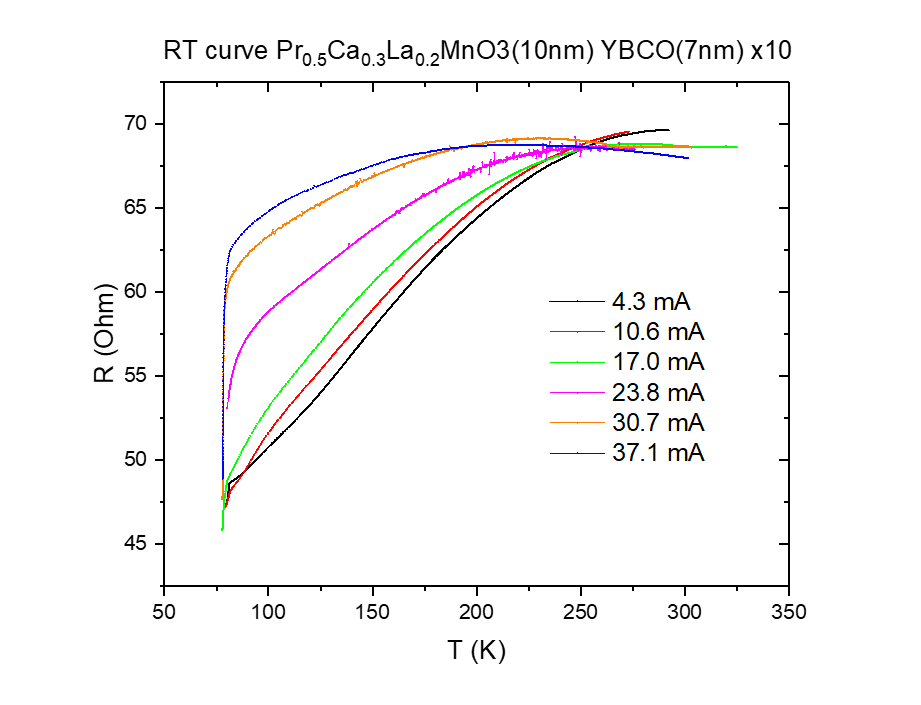
\includegraphics[width=100mm]{Bilde1.png}
\caption{Resistance as function of temperature from 298K (room temperature) to 80K with liquid nitrogen as the cooling medium. The black graph is the graph got from 4.3mA, the red graph corresponds to 10.6mA, the green graph is 17.0mA, the magenta is 23.8mA, the orange is 30.7mA and finally the blue one is 37.0mA. The resistance is normalized with respect to room temperature. \label{fig:res_norm}}
\end{figure}
Further we used the monogomery technique to turn the sample, and saw how the resistance was with current flowing perpendicular to the defect, and the result is plotted in figure (\ref{fig:res}). As we can see the initial resistance is higher when the current flows perpendicular to the defect than parallel to it. 
\begin{figure}[h]
\centering
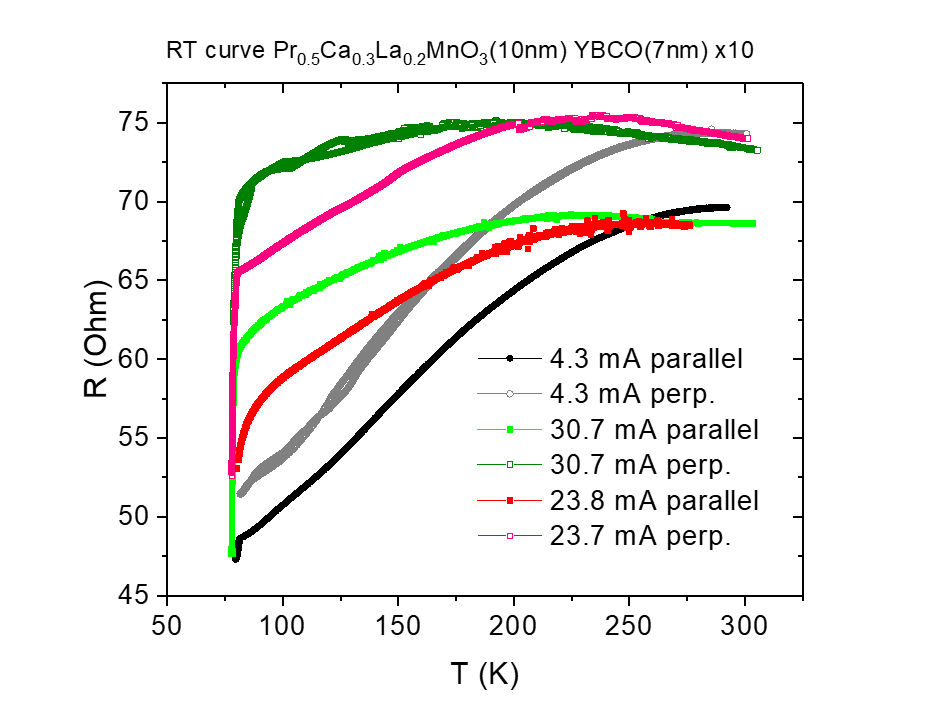
\includegraphics[width=100mm]{Bilde2.png}
\caption{Resistance as function of temperature from 298K (room temperature) to 80K with liquid nitrogen as the cooling medium. The black graph is the graph got from 4.3mA, the red graph corresponds to 10.6mA, the green graph is 17.0mA, the magenta is 23.8mA, the orange is 30.7mA and finally the blue one is 37.0mA. \label{fig:res}}
\end{figure}

Moreover we studied how the current was changing as the temperature decreased for both the parallel and perpendicular case, and the result is shown in figure (\ref{fig:cur}). The legend indicated the initial current. We see that the currents are roughly the same in both cases, so there is enough to study one of them, but where the two higher currents increase for low temperatures, the lower current seems to decrease. It would therefore be interesting to see how the current graphs are behaving when we normalize them, and a plot of that is presented in figure (\ref{fig:cur_norm}). 
\begin{figure}[h]
\centering
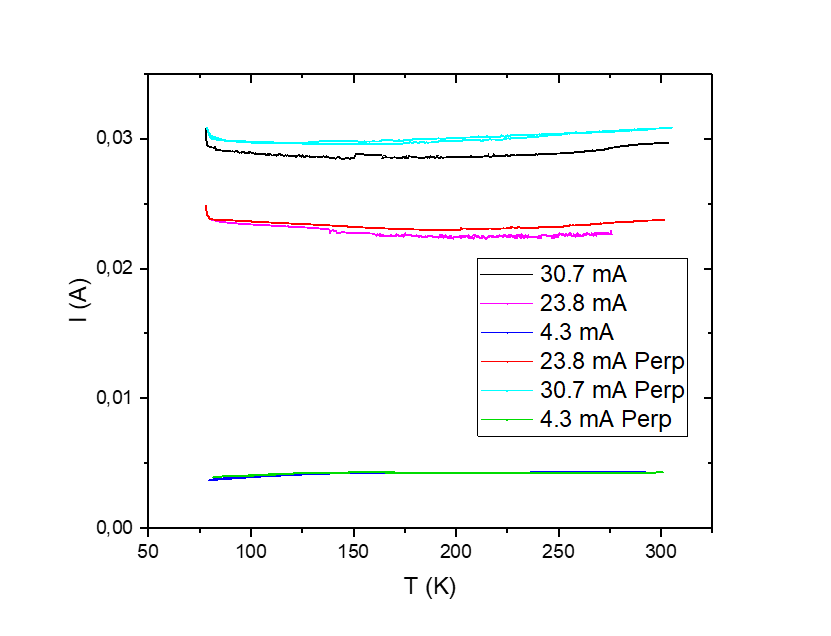
\includegraphics[width=100mm]{Bilde3.png}
\caption{The current as function of temperature with 4.3mA, 23.7mA and 30.7mA as the initial currents for both current flowing parallel and perpendicular to the defect.\label{fig:cur}}
\end{figure}
\begin{figure}[h]
\centering
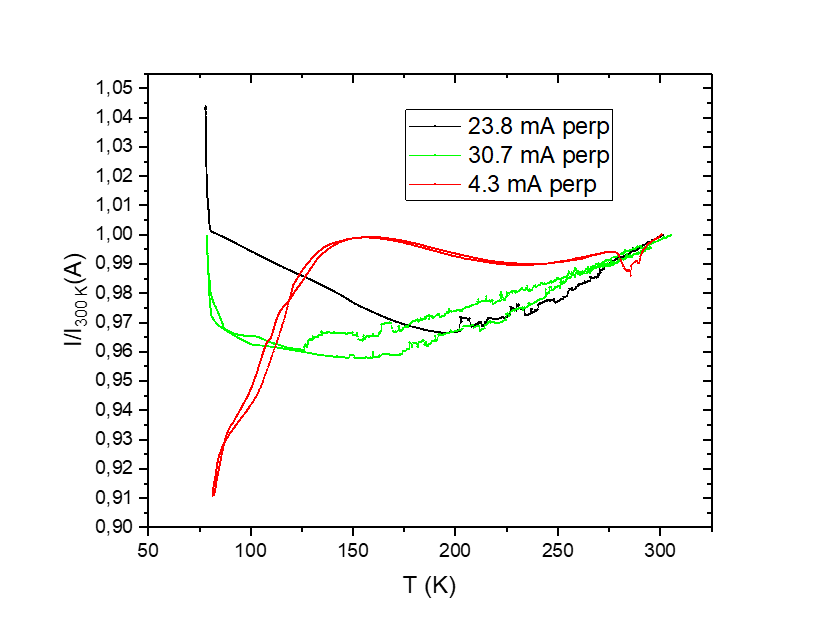
\includegraphics[width=100mm]{Bilde4.png}
\caption{The current as function of temperature with 4.3mA, 23.7mA and 30.7mA as the initial currents for the perpendicular case. The currents are normalizing with respect to the initial current.\label{fig:cur_norm}}
\end{figure}
As we can see, the lower current graph is actually decreasing for low temperatures, which makes no sense according to Ohm's law. This is discussed in section \ref{Sec:Discussion}.

\section{Discussion} \label{Sec:Discussion}
In figure (\ref{fig:rutherfordRTallI}) and (\ref{fig:rutherfordRTlowI}) we got transition at higher temperature when we had $I=0.7A$ than $T=0.2A$, which makes no sense. The reason is not clear, but it could be that we increased the temperature too fast, or maybe we got an unusual hysteresis. We have a small distance between the temperature sensor and the sample, which causes some delay in temperature information, i.e, the temperature gotten from the sensor is slightly different from the actual temperature of the sample. Anyway in figure (\ref{fig:rutherfordRT}) the curves behave as expected. 

Furthermore in figure (\ref{fig:moi2d1}) we saw that the \chem{MgB_2} was superconducting at 3.7K, but surprisingly Niobium is dark and indicates that it is not superconducting, which is strange. Maybe the temperature is wrong. Moreover the figure (\ref{fig:moi2d2}) the sample looks superconducting on the edges of the \chem{MgB_2} core. The reason is that the magnetism has penetrated the core from both sides. 

In figure (\ref{fig:res}) the resistance was apparently higher when the current flowed perpendicular to the defect, than when it flowed parallel to the defect. This is probably because the contacts are more resistive in this case, ideal (with the same contacts) the resistance should be the same. Therefore it would be better to normalize all graphs with respect to the initial resistance to make the comparison easier. We also saw that the higher currents tend to be resisitive for lower temperatures, which causes a big drop when the critial temperature is reached. 

\section{Conclusion} \label{Sec:Conclusion}
Need to conclude after finishing the discussion.

\ack{This report was written as the final report in the course FYS4180 - Experimental methods in physics, fall 2017, University of Oslo.}

\section{References}
\begingroup
\renewcommand{\section}[2]{}
\begin{thebibliography}{}
\bibitem{jsap}
  Discovery of the new superconductor \chem{MgB_2} and its recent development. 
  Y. Zenitani, J. Akimitsu. 
  JSAP International No.6 (July 2002)
  \url{https://www.jsap.or.jp/jsapi/Pdf/Number06/04_CuttingEdge1.pdf}
\bibitem{nature}
  Superconductivity at 39 K in magnesium diboride. 
  J. Nagamatsu, N. Nakagawa, T. Muranaka, Y. Zenitani, J. Akimitsu. 
  Nature 410, 63–64 (01 March 2001)
  \url{https://www.nature.com/articles/35065039}
\bibitem{fnal}
  Development of Rutherford-type Cables for High Field Accelerator Magnets at Fermilab.
  N. Andreev, E. Barzi, E. Borissov, L. Elementi, V.S. Kashikhin, V. Lombardo, A. Rusy, D. Turrioni, 
R.Yamada, A.V. Zlobin.
   Fermi  National  Accelerator  Laboratory,  Batavia, IL 60510 USA (28 August 2016)
  \url{http://lss.fnal.gov/archive/2006/conf/fermilab-conf-06-323-td.pdf}
\bibitem{harvard}
  Superconductivity at 93 K in a new mixed-phase Y-Ba-Cu-O compound system at ambient pressure.
  Wu, M. K.; Ashburn, J. R.; Torng, C. J.; Hor, P. H.; Meng, R. L.
  Physical Review Letters (ISSN 0031-9007), vol. 58, (2 March 1987), p. 908-910.
  \url{http://adsabs.harvard.edu/abs/1987PhRvL..58..908W}
\end{thebibliography}
\endgroup
\nocite{*}

\bibliographystyle{compj}
\bibliography{ModellingBidders}


\end{document}